\documentclass{article}
\usepackage[utf8]{inputenc}
\usepackage{amssymb,amsmath,amsthm}
\usepackage{enumerate}
\usepackage[left=.75 in, right=.75 in,top=.75 in, bottom=.75 in]{geometry}
\usepackage{fancyhdr}
\usepackage{bm}
\usepackage{graphicx}
\usepackage{subfig}
\usepackage{parskip}

\graphicspath{ {img/} }

\pagestyle{fancy}
\fancyhf{}
\fancyhead[L]{Statistical Modeling and Analysis of SST-Pyr Synapses}
\fancyhead[R]{Page \thepage}
\renewcommand{\headrulewidth}{0.4pt}

\setlength{\parskip}{2mm}

\def\Pr{\textbf{Pr }}
\def\Var{\textbf{Var}}
\def\E{\textbf{E}}

\newcommand{\rv}[1] {
\text{$\bm{#1}$}
}

\DeclareMathOperator{\bern}{Bern}

\providecommand{\norm}[1]{\left\Vert#1\right\Vert}

\author{Taisuke Yasuda}

\begin{document}

\begin{center}
  {\LARGE Statistical Modeling and Analysis of SST-Pyr Synapses} \\
  \vspace{10pt}
  {Taisuke Yasuda \qquad 10/01/2016}
\end{center}

\section{Results}
\subsection{Summary}
Our studies show that the observed data is best explained by a distribution of postsynaptic amplitudes over contacts with a high variance. We first find that the simple model obtained by assuming that the release probabilities, which we refer to as $p$, and response amplitudes, which we refer to as $q$, of each contact are the same does not sufficiently explain the data obtained from the experiment. We then find that when we take the response amplitudes across contacts to have a uniform distribution with large width parameter, we recover a model that explains the data well, as measured by QQ plots.

\subsection{Assuming constant $p$ and constant $q$ at each contact}
The first attempt at inferring the underlying biology from the observed data was to build a statistical model for a single trial (i.e.\ a single spike in a train of 10) assuming that the release probabilities and postsynaptic response amplitudes were all the same for every one of the $N$ contacts that contribute to the observed summed amplitude. We constructed a model that depended on four parameters: the number of contacts $N$, a constant variance $\sigma^2$ at each contact, a constant release probability $p$ at each contact, and a constant response amplitude $q$ at each contact. Although these assumptions are not biologically reasonable for every synapse, they help us assess whether the frequency at which the extremely large amplitudes occur is simply a result of the structure of the statistical model or not.

\subsubsection{Visualization of the model via histograms}
We can start a first investigation of this model by visualizing simulations of the model with histograms. In this section, along with an initial assessment of the data and the statistical model, we develop methodologies that we will use later to assess a different model. In order to simulate the model, we estimate parameters using the data that we collected. When we assume that the release probabilities are all constant for each contact, we can estimate the release probability using the failure rate $p_f$, by
\[
  p = 1 - \sqrt[N]{p_f}.
\]
Given this release probability and the sample mean $\hat{\mu}$ of the observed data, we estimate the response amplitude by
\[
  q = \frac{\hat{\mu}}{Np}.
\]
Finally, we estimate the parameter variance using the sample variance $s^2$ of the observed data by
\[
  \sigma^2 = \frac{1}{N}s^2.
\]
The justifications for these estimations are shown in the methods section. Note that we do not make an estimation on $N$, yet all of our other estimations rely on knowledge of $N$. We attempted an estimation of $N$ via clustering and fitting a mixture of Gaussians model, but the results were inconclusive. Thus, we simulate data for all $N$ in the range $N = 4$ to $N = 11$, which is a reasonable range to assume given the range of possible $N$ seen from reconstructions of the cells.

Using the parameters, we simulate the model and plot the results in a histogram. Figure 1 shows an example of a simulation that captures the shape of the observed data fairly well for some values of $N$, at least on first sight. However, goodness of fit is difficult to assess just with the human eye. Therefore, we use QQ plots to assess the goodness of fit of these models.
\begin{figure}[h]
  \centering
  \caption{Simulations assuming constant parameters}
  \includegraphics[width=1.0\textwidth]{10sept2015f-4}
\end{figure}

\subsubsection{Visualization via QQ plots}
QQ plots allow us to directly compare the observed data with our proposed model by sampling from the proposed model many times and comparing the quantiles of this sampling with the quantiles of the observed data. Because the simulated percentage of zeros matches the percentage of zeros of the observed data by construction, we will just analyze the nonzero values (Figure 2).

\begin{figure}[h]
  \centering
  \caption{QQ plots for constant parameter model}
  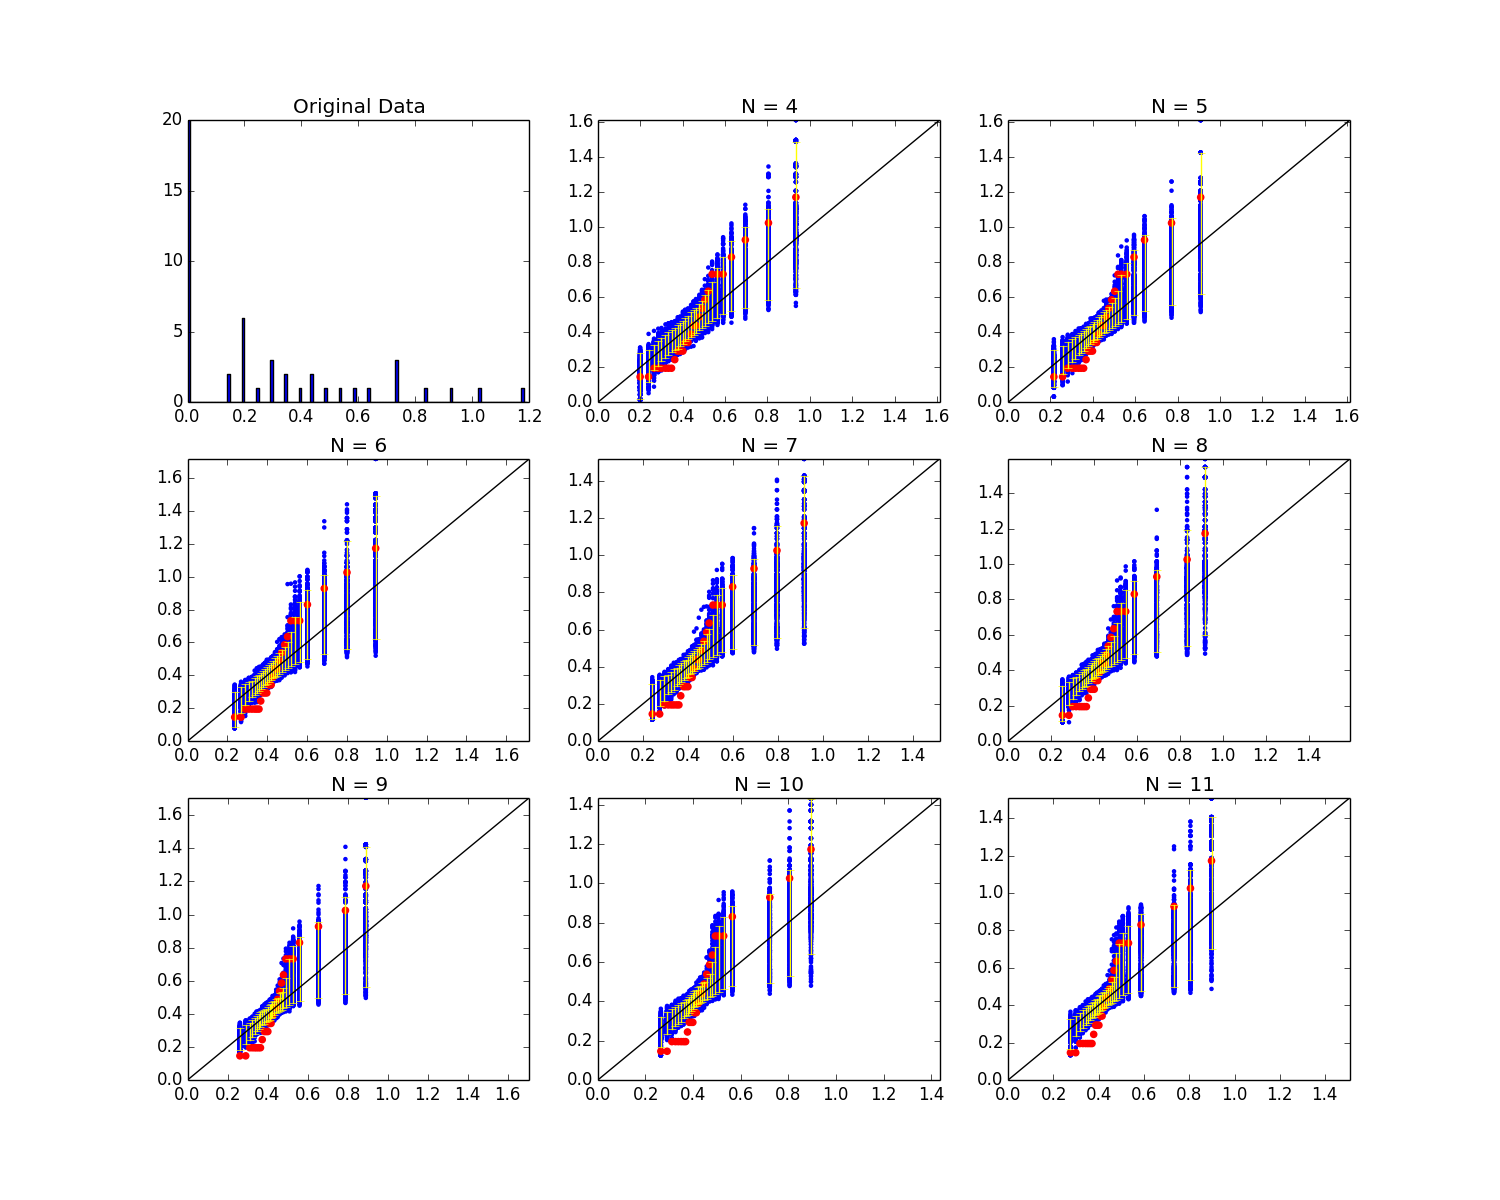
\includegraphics[width=1.0\textwidth]{10sept2015f-4-qq}
\end{figure}

In this figure, we show the QQ plot for the same cell as Figure 1, with the same range of values for $N$. In the QQ plot, the blue points indicate the simulated values from the constant parameter model, the yellow points indicate the $95\%$ confidence band, and the red points indicate the observed data, all plotted against the quantiles of the simulated values. With this analysis, we see that though the largest events of the observed data are towards the high end of the simulated values, they are still within the $95\%$ confidence band. However, the lower values are outside of the $95\%$ confidence band, so we cannot say that this model truly explains the data well: the problem is to explain the high amplitude events in relation to the rest of the data.

Upon inspecting the QQ plots for other cells, we see that high amplitude events are actually explained fairly well. However, in general, this model seems to sacrifice the goodness of fit of the events at lower amplitudes, consistently overestimating the value of the quantile. Intuitively, we should have expected this result: because we set all the contacts to have the same amplitude, the probability of the occurrence of these particular amplitudes and their multiples becomes higher.

\subsection{Assuming a uniform distribution on $q$}
Apparently, setting everything as constant does not explain the data sufficiently, as shown by the QQ plot analysis. The next simplest assumption we could make is to assume some other distribution on $p$ or $q$ while keeping the other constant. By perturbing the parameters of these assumed distributions and seeing how the resulting distribution of $\rv{A}$ changes, we can possible gain more understanding on the relationship between the parameters and the resulting distribution. Thus, we assume a uniform distribution on $q$, where we assume that the $q_j$s are drawn from a range $[a,b]$ with equal probability. To simplify this exploration, we will simply draw $N$ equidistant $q_j$s from an assumed range. We should still satisfy the constraints given by the failure rate $p_f$ and sample mean $\hat{\mu}$, so we derive expressions for $q_j$ that comply to these constraints. Because we kept $p_j$ all constant, we can simply take the choice from before, where $p_j = p = 1 - \sqrt[N]{p_f}$ for all $1 \leq j \leq N$. To make a suitable choice for $q_j$, we require that the mean of the uniform distribution match the mean of the observed data and choose the distribution to have a width $w$, which is a parameter we control.

\begin{figure}[h]
  \centering
  \caption{Choosing the $q_j$ from a distribution with mean $\hat{\mu}/Np$ and width $w$.}
  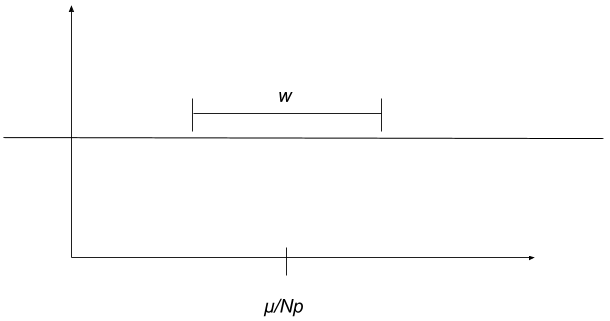
\includegraphics[width=0.5\textwidth]{uniform}
\end{figure}

To make a suitable choice for $q_j$, first note that:
\[
  \rv{\bar{A}} = \sum_{j=1}^N p_jq_j = p\sum_{j=1}^N q_j \iff \frac{1}{N}\sum_{j=1}^N q_j = \frac{\rv{\bar{A}}}{Np}
\]
Then, if we decide the $q_j$s to span a width $0 \leq w < 2\frac{\rv{\bar{A}}}{Np}$, then we can choose $q_j = \frac{w}{N-1}j + \frac{\rv{\bar{A}}}{Np} - \frac{w}{2}$ for $j \in \{0,1,...,N-1\}$.

Now, we will take a random trial of a random cell with a random $N$ to see how imposing this structure on $q_j$ will affect the resulting QQ plot for various values of $w$ (Figure 3).

\begin{figure}[h]
  \centering
  \caption{QQ plots for uniformly distributed $q$, varying the distribution width}
  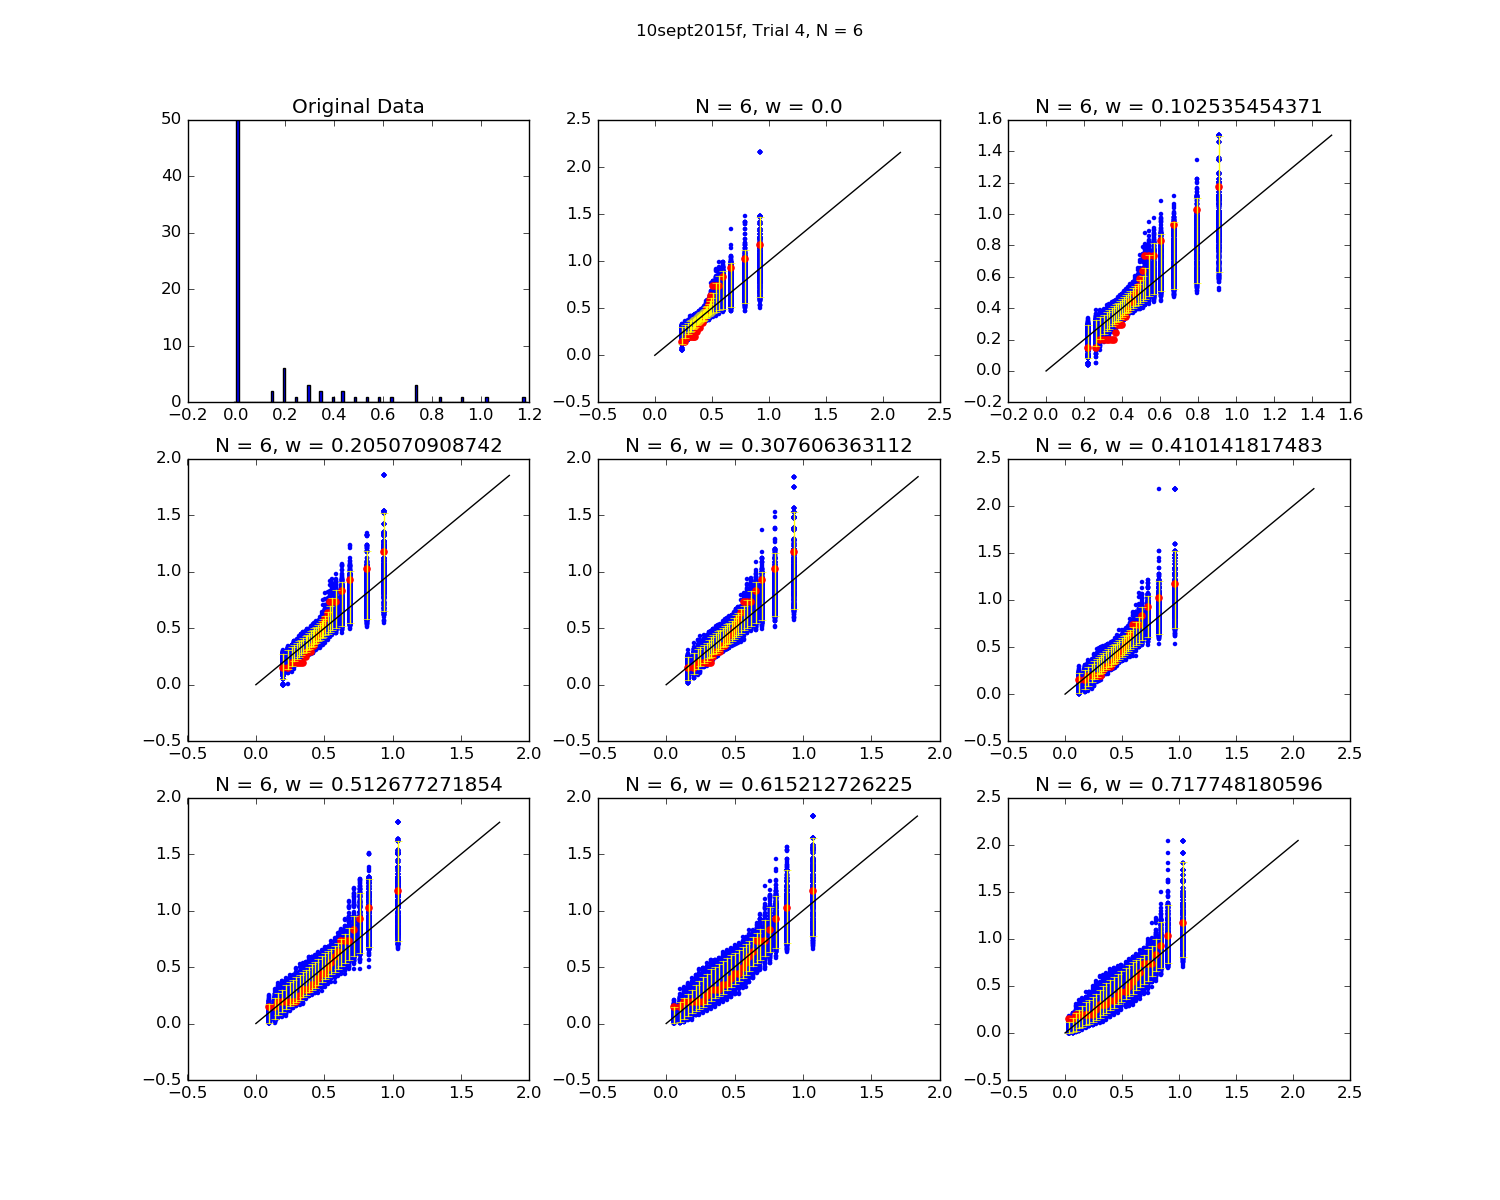
\includegraphics[width=1.0\textwidth]{10sept2015f-4-6-qq}
\end{figure}

In Figure 4, we actually see that as we take the width of the uniform distribution $w$ to be larger and larger, we bring the observed distribution closer and closer to the simulated distribution! In fact, for large enough values of $w$, this puts the observed data within the $95\%$ confidence intervals of the simulated data. This effect was seen in general across all trials and guesses for $N$s for this particular cell. The observation that a particular effect of changing the $q$s on the distribution would hold across trials is not surprising, as we expect the $q$s of a cell to stay the same across trials. However, because this effect holds across our guesses for $N$s of a cell, we conclude that this is a fundamental characteristic of the data. When we try these simulations on more cells, this effect holds for them as well, sometimes achieving particularly excellent results (Figure 4).

\begin{figure}[h]
  \centering
  \caption{An example of an excellent fit}
  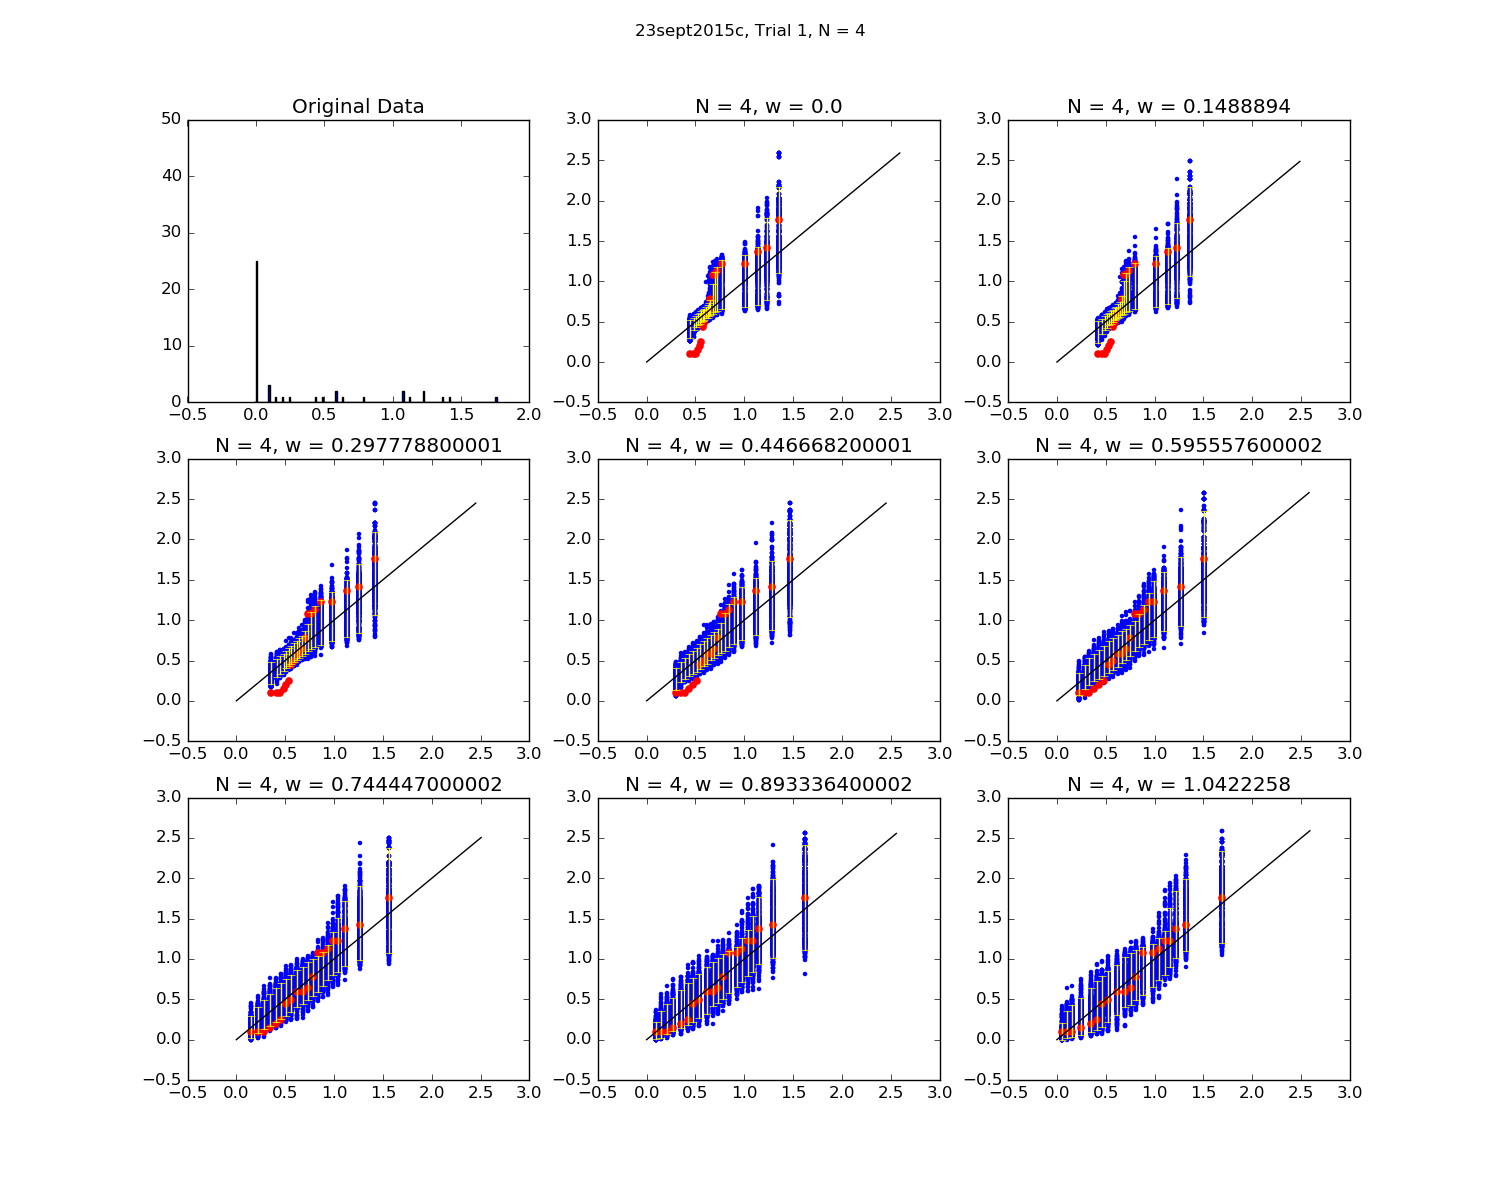
\includegraphics[width=1.0\textwidth]{23sept2015c-1-4-qq}
\end{figure}

The existence of these excellent fits suggest that this is an optimal method of explaining the data -- we expect that fitting the data even better is just a matter of tuning the parameters initialized from the equidistant $q_j$s with width $w$. In Figure 5, we show what the simulations of these fits look like on the same cell as before.

\begin{figure}[h]
  \centering
  \caption{Simulations of a successful fit}
  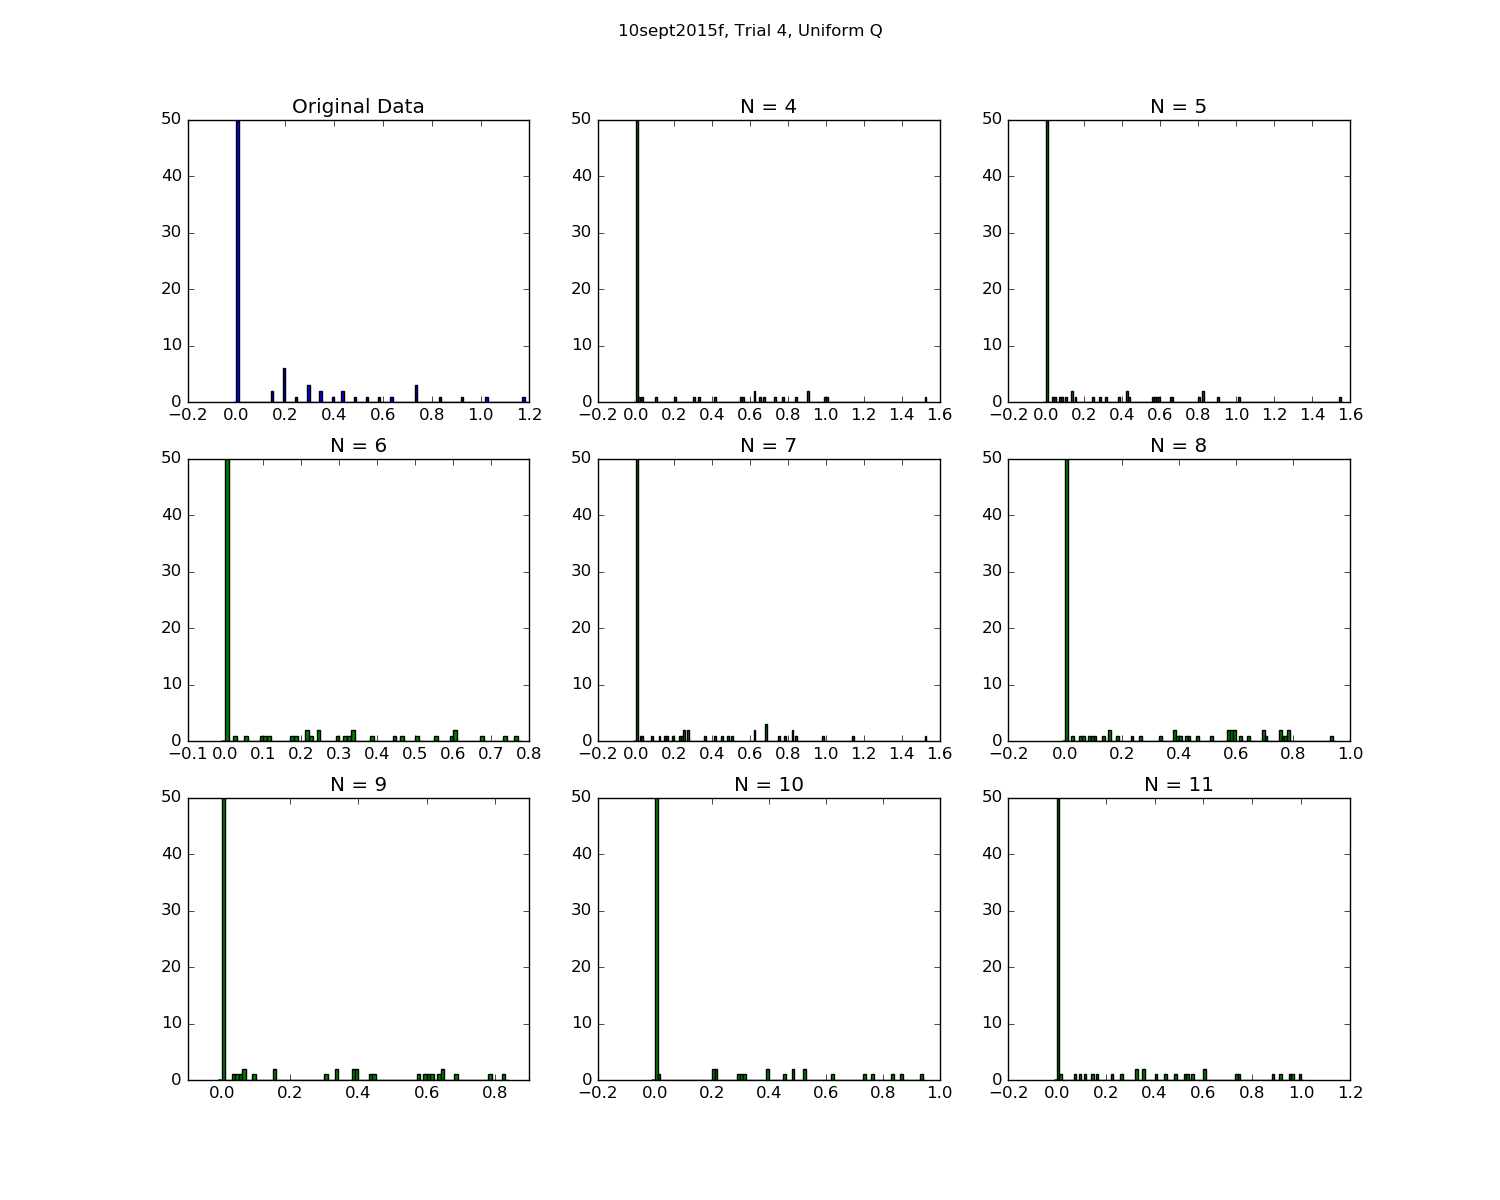
\includegraphics[width=1.0\textwidth]{10sept2015f-4-uq}
\end{figure}

\section{Methods}

\subsection{Underlying statistical model of one trial}
We first build a statistical model based on the underlying biology of the observed measurements:
\[
  \rv{A} = \sum_{j=1}^N \rv{A}_j, \rv{A}_j = \begin{cases}
    N(q_j,\sigma_j) & \text{if $\rv{S}_j = 1$} \\
    0 & \text{if $\rv{S}_j = 0$}
  \end{cases}, \rv{S}_j = \bern(p_j)
\]
In this model, $\rv{A}$ represents the overall response amplitude that we observe and is the sum of $\rv{A}_j$ where $j$ takes on integers from $1$ to $N$. Each $\rv{A}_j$ represents the response amplitude of an individual synaptic contact and $j$ indexes the synaptic contacts. The response of an individual synaptic contact depends on its release success, so we model release success with a latent Bernoulli variable $\rv{S}_j$ with parameter $p_j$ representing the release probability of the particular contact. If contact $j$ succeeds in release, e.g. $\rv{S}_j = 1$, then $\rv{A}_j$ is normally distributed with mean $q_j$ and standard variation $\sigma_j$. If contact $j$ fails to release, e.g. $\rv{S}_j = 0$, then $\rv{A}_j = 0$.

\subsection{Initial analysis of the model}

\subsubsection{Trying all constant}
A simple way to visualize this statistical model is to assume some number of contacts $N$, assume some uniform standard deviation $\sigma$, mean response $q$, and release probability $p$ for every one of the $N$ contacts. Under these assumptions, we can make reasonable estimate the parameters $p$, $q$, and $\sigma$ from the data.

\subsubsection{Estimation of Parameters}
We first estimate $p$ using the observed failure rate $p_f$. If a cell responds with an amplitude of $0$, then this happens exactly when all of its $N$ contacts fail to release. Then, since all the contacts have the same release probability $p$ under our assumptions, we conclude the following value for $p$:
\[
  p_f = (1-p)^N \iff \sqrt[N]{p_f} = 1 - p \iff p = 1 - \sqrt[N]{p_f}
\]
Next, we estimate $q$ using the mean response $\rv{\bar{A}}$. We can compute the expectation of our observed random variable $\rv{A}$ as follows:
\begin{align*}
    \E[\rv{A}] &= \E[\sum_{j=1}^N \rv{A}_j] = \sum_{j=1}^N \E[\rv{A}_j] \\
    &= \sum_{j=1}^N \E[\rv{A}_j \mid \rv{S}_j = 1] \Pr[\rv{S}_j = 1]
    + \E[\rv{A}_j \mid \rv{S}_j = 0] \Pr[\rv{S}_j = 0] \\
    &= \sum_{j=1}^N \E[N(q,\sigma)]p + 0 = \sum_{j=1}^N qp = Npq
\end{align*}
Since we have assumed $N$ and estimated $p$ and $\rv{\bar{A}} \approx \E[\rv{A}]$, we have an estimate for $q$. Finally, we make an estimate on $\sigma$ using the variance of the distribution $\Var(\rv{A})$. Since we have that each of the contacts are independent of one another, by the linearity of variance of independent random variables, we have that $\Var(\rv{A}) = \sum_{j=1}^n A_j$. In particular, if $\sigma$ is constant for all the contacts, then $\sigma^2 = \frac{1}{N} \Var(\rv{A})$

\subsection{Assuming distributions on $q$}
Apparently, setting everything as constant does not explain the data sufficiently, as shown by the QQ plot analysis. The next simplest thing we could do is to assume some other distribution on $p$ or $q$ while keeping the other constant. By perturbing the parameters and see how the resulting distribution of $A$ changes, we can possible gain more understanding on the relationship between the parameters and the resulting distribution.

In doing this analysis, it is actually much easier to perturb $q$ while keeping $p$ constant, since we don't have the constraint of $p_f$ -- we can in fact find closed form solutions to the values of $q_j$ we should use for very simple cases.

\subsubsection{Uniform Distribution}
The simplest distribution that we could assume on $q$ is the uniform distribution, where we assume that  the $q_i$s are drawn from a range $[a,b]$ with equal probability. To simplify this exploration, we will simply draw $N$ equidistant $q_j$s from an assumed range. We should still satisfy the constraints given by $p_f$ and $\rv{\bar{A}}$, so we derive expressions for $q_j$ that comply to these constraints. Because we kept $p_j$ all constant, we can simply take the choice from before, where $p_j = p = 1 - \sqrt[N]{p_f}$ for all $1 \leq j \leq N$. To make a suitable choice for $q_j$, first note that:
\[
  \rv{\bar{A}} = \sum_{j=1}^N p_jq_j = p\sum_{j=1}^N q_j \iff \frac{1}{N}\sum_{j=1}^N q_j = \frac{\rv{\bar{A}}}{Np}
\]
Thus, we just need to choose $q_j$ to be an arithmetic progression with mean $\frac{\rv{\bar{A}}}{Np}$. If we decide the $q_j$s to span a width $w < 2\frac{\rv{\bar{A}}}{Np}$, then we we choose $q_j = \frac{w}{N-1}j + \frac{\rv{\bar{A}}}{Np} - \frac{w}{2}$ for $j \in \{0,1,...,N-1\}$. Note that when $j = 0$, $q_j = \frac{\rv{\bar{A}}}{Np} - \frac{w}{2}$ and when $j = N-1$, $q_j = \frac{\rv{\bar{A}}}{Np} + \frac{w}{2}$.

Now, we will take a random trial of a random cell with a random $N$ to see how imposing this structure on $q_j$ will affect the resulting QQ plot for various values of $w$ (Figure 3).

\begin{figure}[h]
  \centering
  \caption{QQ plots for uniformly distributed $q$, varying the distribution width}
  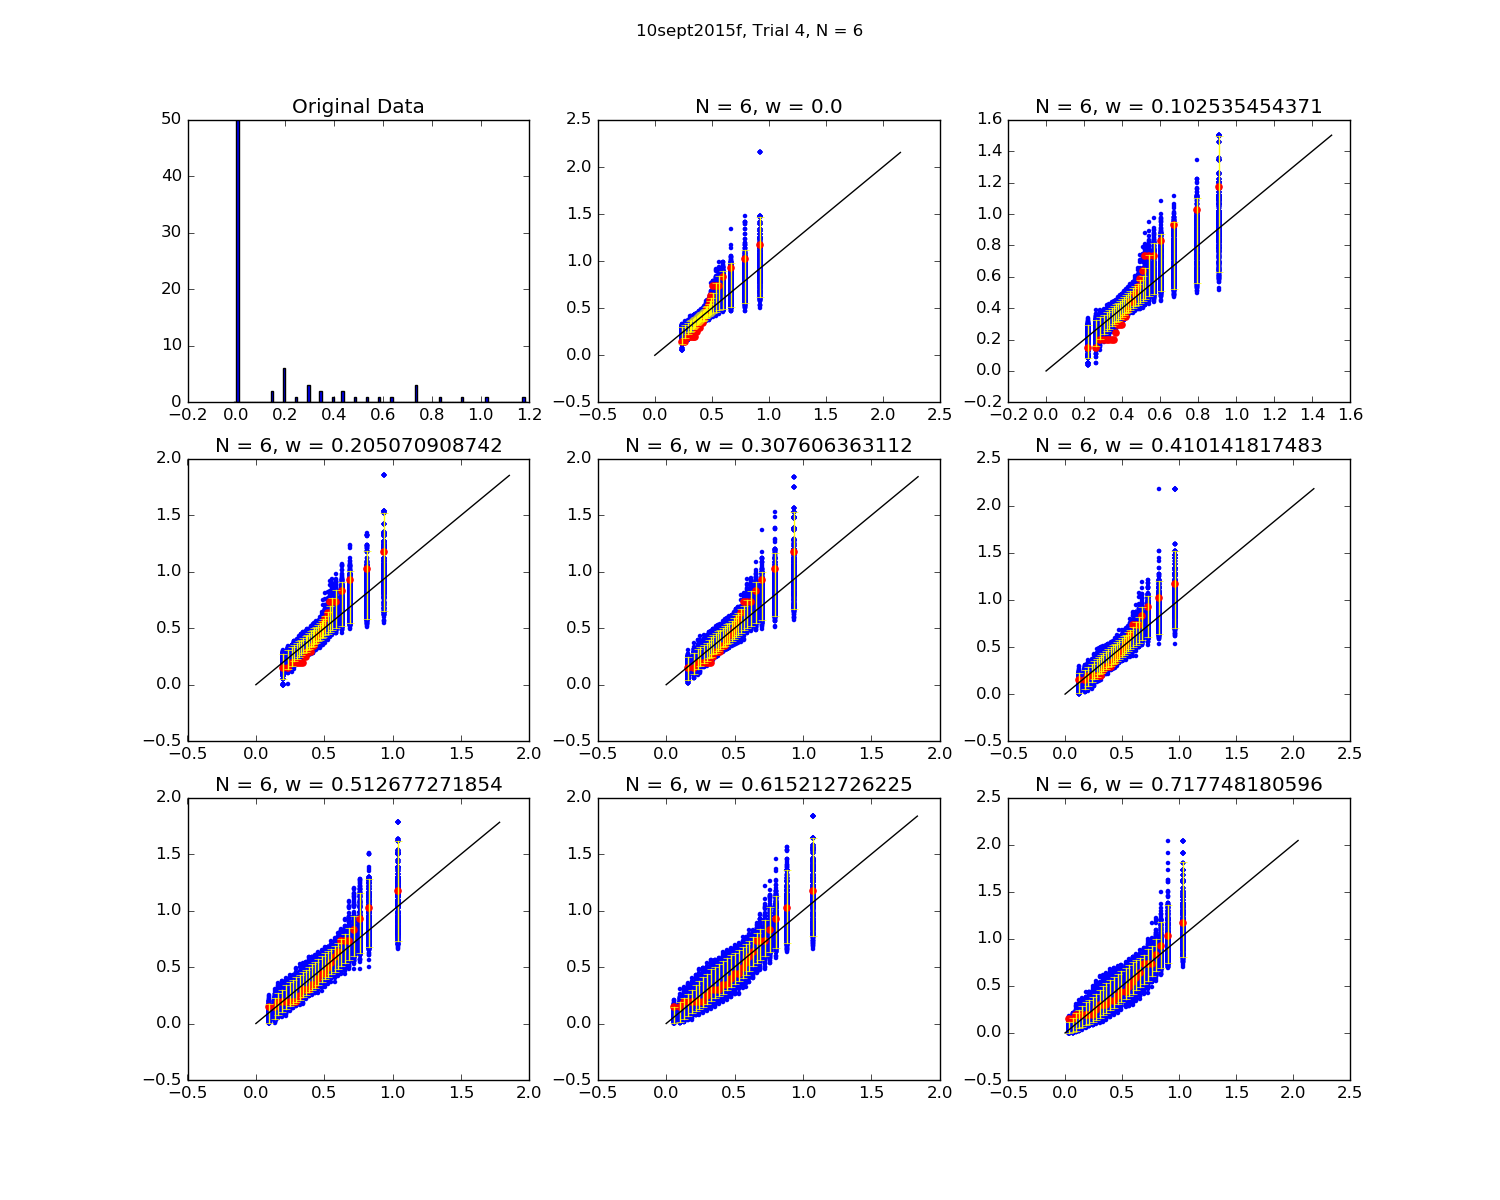
\includegraphics[width=1.0\textwidth]{10sept2015f-4-6-qq}
\end{figure}

In Figure 3, we actually see that as we take the width of the uniform distribution $w$ to be larger and larger, we bring the observed distribution closer and closer to the simulated distribution! In fact, for large enough values of $w$, this puts the observed data within the $95\%$ confidence intervals of the simulated data. This effect was seen in general across all trials and guesses for $N$s for this particular cell. The observation that a particular effect of changing the $q$s on the distribution would hold across trials is not surprising, as we expect the $q$s of a cell to stay the same across trials. However, because this effect holds across our guesses for $N$s of a cell, we conclude that this is a fundamental characteristic of the data. When we try these simulations on more cells, this effect holds for them as well, sometimes achieving particularly excellent results (Figure 4).

\begin{figure}[h]
  \centering
  \caption{An example of an excellent fit}
  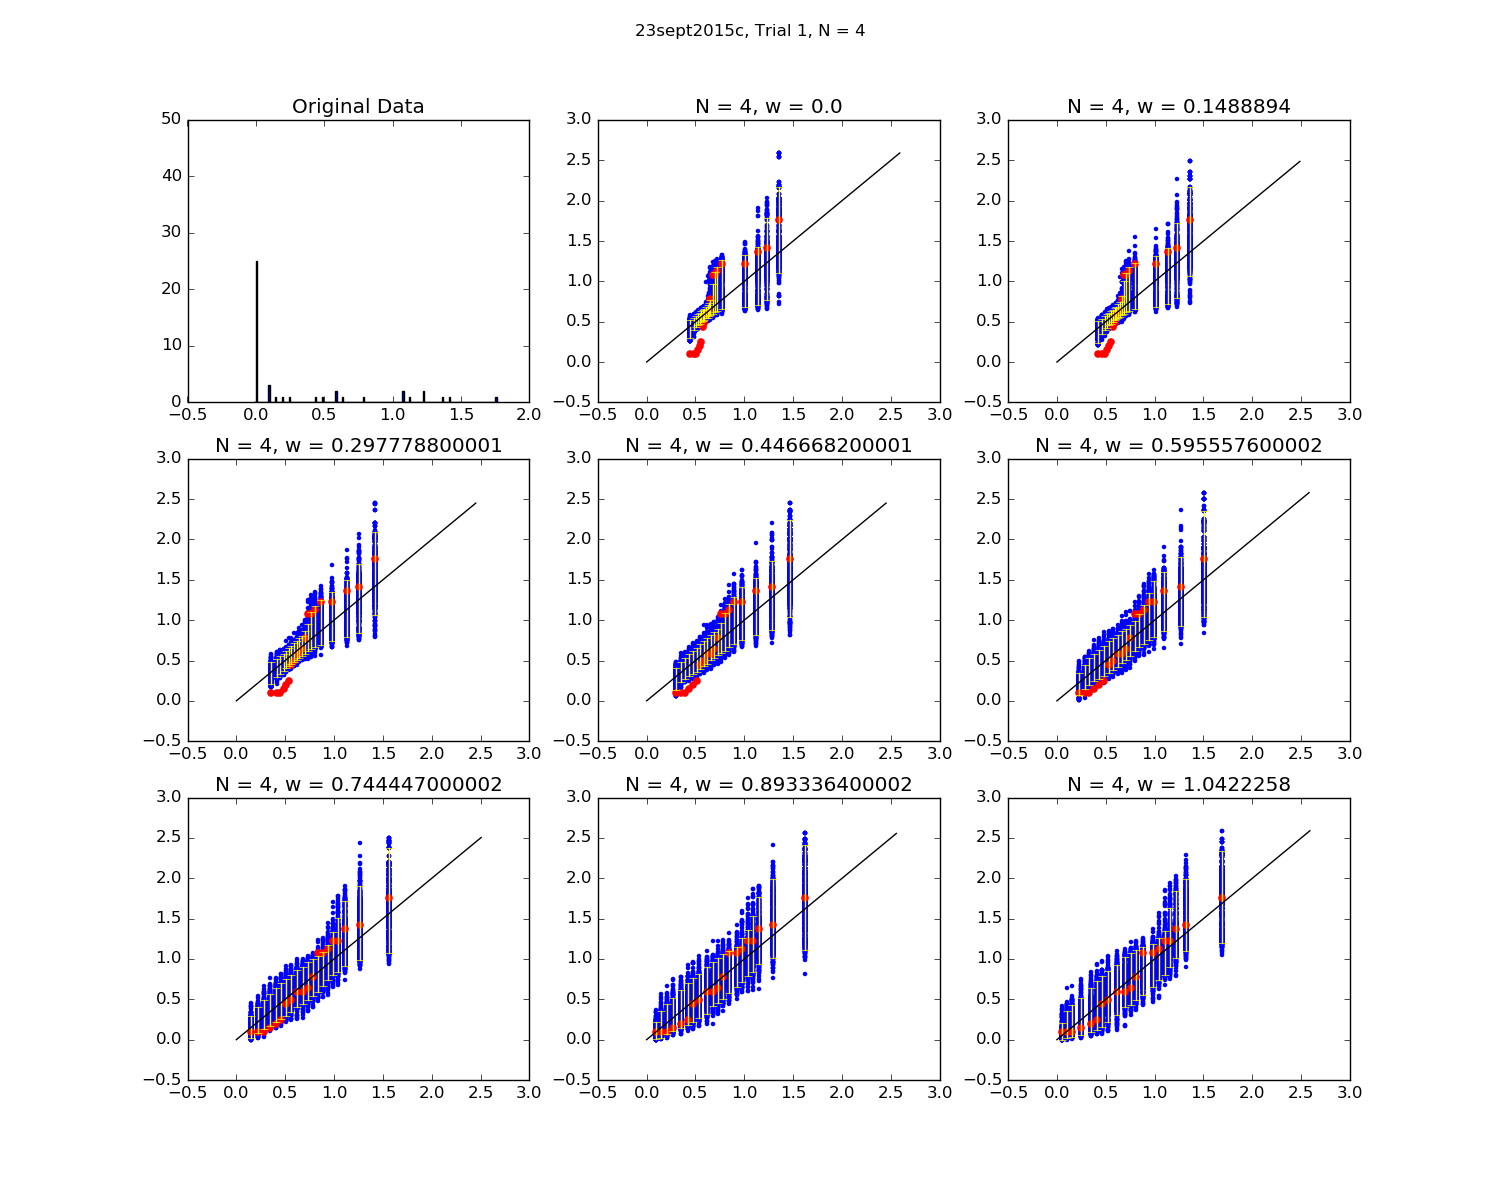
\includegraphics[width=1.0\textwidth]{23sept2015c-1-4-qq}
\end{figure}

The existence of these excellent fits suggest that this is an optimal method of explaining the data -- we expect that fitting the data even better is just a matter of tuning the parameters initialized from the equidistant $q_j$s with width $w$. In Figure 5, we show what the simulations of these fits look like on the same cell as before.

\begin{figure}[h]
  \centering
  \caption{Simulations of a successful fit}
  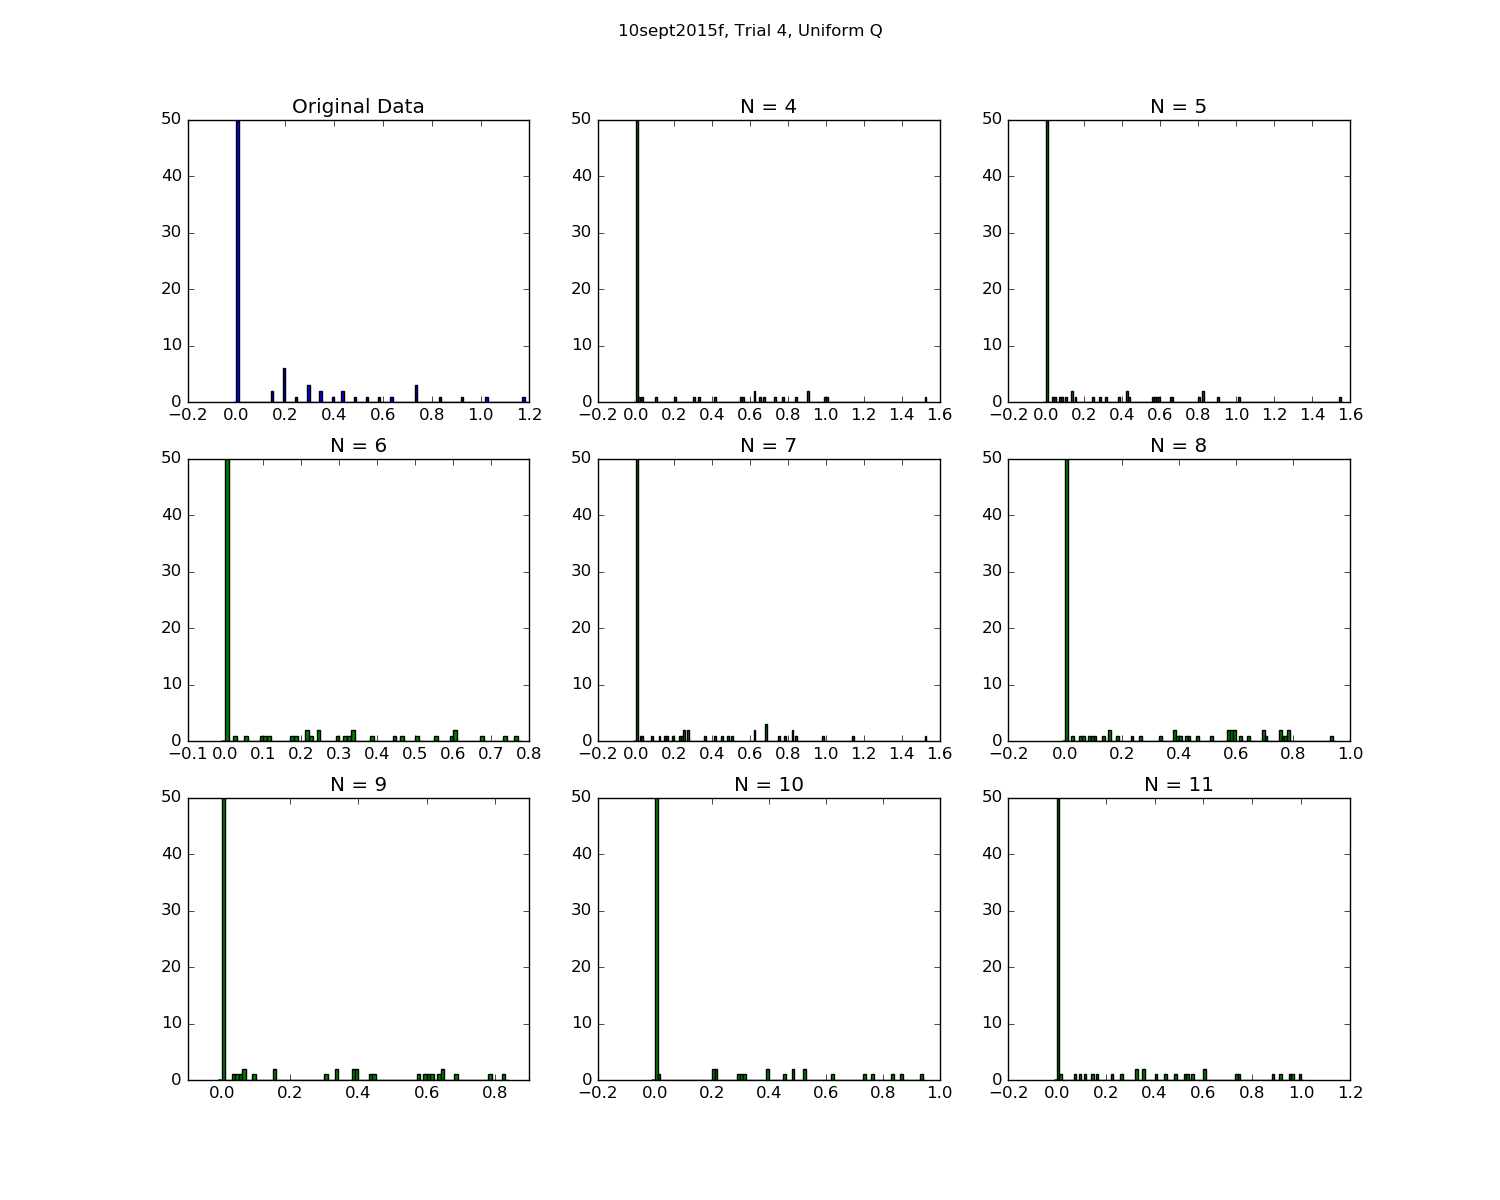
\includegraphics[width=1.0\textwidth]{10sept2015f-4-uq}
\end{figure}

\subsection{Statistical model for the entire experiment}
At this point, we are fairly confident that we can explain single trials of events. However, we have further constraints to satisfy -- for the trials that we know belong to the same cell, we know that the $q_j$s should be the same. Thus, we should be able to find a single set of $q_j$s for all of the trials for each cell. If we keep our assumption that $p$ is constant for each trial, then we can find this value in exactly the same way as we did for the analysis of single trials. We proceed as follows: we first estimate the mean value of $q_j$ from the whole data set as before, with the formula $\frac{1}{N}\sum_{j=0}^N q_j = \frac{\rv{\bar{A}}}{Np}$. We then find the $q_j$ found by the arithmetic progression and repeat the QQ plot measurement for each trial with their own $p$ values, estimated as before with the formula $1 - \sqrt[N]{p_f}$.

\section{Technical Appendix}

\end{document}
